\documentclass{article}
\usepackage[utf8]{inputenc}

\usepackage{lmodern}  % for bold teletype font
\usepackage{amsmath}  % for \hookrightarrow
\usepackage{xcolor} 
\usepackage{listings}
\usepackage{listings-rust}
\usepackage{tcolorbox}
\usepackage{float}
\floatstyle{boxed} 
\restylefloat{figure}

\lstset{
  basicstyle=\ttfamily,
  columns=fullflexible,
  frame=single,
  breaklines=true,
  postbreak=\mbox{\textcolor{red}{$\hookrightarrow$}\space},
}



\newcommand{\lstfont}[1]{\color{#1}\scriptsize\ttfamily}

% CUDA Coloring

\lstdefinestyle{MyCUDAStyle} {
    language=[ANSI]C++,
    showstringspaces=false,
    %backgroundcolor=\color{black!90},
    %basicstyle=\lstfont{white},
    %identifierstyle=\lstfont{white},
    keywordstyle=\lstfont{orange!100},
    %numberstyle=\lstfont{white},
    stringstyle=\lstfont{cyan},
    commentstyle=\lstfont{yellow!30},
    emph={
        cudaMallocManaged, cudaFree, cudaDeviceSynchronize, cudaMemcpy, cudaMemcpyHostToDevice, cudaMemcpyDeviceToHost,
        __global__, __shared__, __device__, __host__, <<<, >>>,
        __syncthreads,
    },
    emphstyle={\lstfont{blue!100}},
    breaklines=true
}

\title{Validating The Bitcoin Blockchain on GPU}
\author{Daniel Volya, Marhsall Rawson}
\date{April 2021}


\begin{document}
\maketitle

\begin{abstract}
    The project consists of two primary goals: 1) implement kernels that validate several blocks' hash in the Bitcoin Blockchain in parallel, and 2) investigate using the open-source Vulkan standard as an alternative to CUDA. When compared to an equivalent sequential program run on the CPU, the open source tools were approximately 5 times slower than the sequential algorithm, and the proprietary CUDA was  approximately 2 times as fast as the sequential algorithm.
\end{abstract}

\section{Motivation}

Block chains are an emerging technology with possible applications in areas of distributed computing. However, it is not hard to imagine a block chain which grows sufficiently quickly such that a machine which is only connected periodically, could not self validate all the blocks in a reasonable time frame with a sequential algorithm. However, the validation of blocks on a proposed block chain is a parallelizable computation.

While the Bitcoin Blockchain only adds a block approximately every 10 minutes, it provides a good testing ground for a proof of concept because it is well known, easy to get the block data, and uses a SHA256 hash as its validation algorithm, which is likely a similar operation to block chains of the future.

We also decided to use this as a testing ground to compare CUDA and Vulkan, as validating block chains should ideally be able to work on as many GPU's as possible.

\section{Background}
\subsection{Bitcoin Blockchain}

Bitcoin is a digital currency where the transactions are stored on a distributed ledger called a block chain. A block chain is a list of blocks which can be independently verified given the rules of the block chain. With the Bitcoin Blockchain, the header of each block is 80 bytes, and the SHA256(SHA256(header)) is bytes 4 to 36 of the next header. Also, the last 6 bytes of SHA256(SHA256(header)) are 0x00.

\subsubsection{SHA256}

SHA256 is a secure-hash algorithm designed to be computationally expensive to take the inverse and discover the original message. The complete details can be found in the 2002 FIPS publication \textit{Secure Hash Standard}. In summary, the steps are:

\begin{enumerate}
    \item Take a message and pad it to the nearest multiple of 512 bits, where the last 64 bits is the binary representation of message length
    \item Every sequence of 512 bits is considered a block, and the following steps are performed on each block
    \item Take the block and place it into the first 16 slots of an array consisting of 64, 32-bit entries
    \item Compute the remaining slots by performing operations consisting of $\sigma_0$ and $\sigma_1$
    \item Compress the 64, 32-bit entries, into a 8, 32-bit array by using an \texttt{initial\_hash} and $\Sigma_1$, $\Sigma_0$, $Ch$, $Maj$, and the cube root of the first 64 prime numbers. If the block is the first block, then the \texttt{initial\_hash} is taken as the square-root of the first 8 prime numbers.
    \item Add to the result the \texttt{initial\_hash} and set the result as the \texttt{initial\_hash} for the next block iteration (or return it if final block).
\end{enumerate}

\subsection{Vulkan}
Vulkan is a cross platform graphics and compute application programming interface (API) that provides efficient access to modern general purpose graphics processing units (GPGPU). This enables developers to abstract away much of the underlying GPGPU hardware,  and focus on developing the high-level applications and programs. NVIDIA, AMD, Intel, and other industry leaders are conformant with the Vulkan specification, which allows for ``write once, run everywhere” GPGPU code. In the following sections we provide an introduction to the Vulkan, discuss advantages and disadvantages, and introduce the toolchains used for implementing Bitcoin Blockchain Validation.

\subsection{WebGPU}
WebGPU is an API that aims to provide GPGPU hardware access and capabilities on the web. WebGPU works on top of modern GPGPU APIs including Vulkan, D3D12, and Metal. The construction exposes the basic primitives of these low-level APIs to the user. Although the purpose is to enable the web to utilize GPGPU hardware, WebGPU also supports native (non-web) applications. Much of WebGPU's design is motivated by the Vulkan specification, but with the benefit that it works on alternative backends. For this reason, we use WebGPU to develop our blockchain validation, but stick with Vulkan as the primary backend. 

\subsection{Vulkan Specification}

In this section we provide an overview of the Vulkan specification, which serves as a tutorial. Namely, we step through the process of obtaining a GPGPU device to running compute code. We demonstrate examples using Rust bindings of WebGPU. In summary, the steps are:

\begin{enumerate}
    \item Get Instance and Physical Device
    \item Creating Buffers
    \item Establish Bind Groups and Bind Group Layouts (WebGPU specific) 
    \item Declaring Compute Pipeline
    \item Run the program
\end{enumerate}

\subsubsection{Instance and Physical Device Enumeration}

The first step to initialization is to create an \texttt{instance}. The \texttt{instance} tries to load Vulkan from the user's system and obtain available implementations. After an \texttt{instance} is successfully established, the program needs to enumerate all physical devices available on the system that support Vulkan. The following listing demonstrates the procedure.

\begin{lstlisting}[language=Rust, style=boxed]
// Create an instance
let instance = wgpu::Instance::new(wgpu::BackendBit::PRIMARY);
// Enumerate physical devices
let adapter = instance.enumerate_adapters(wgpu::BackendBit::PRIMARY);

let devices: Vec<DeviceInfo> = adapter.map(|a| DeviceInfo { info: a.get_info() }).collect();
\end{lstlisting}

\subsubsection{Creating Buffers}

The standard approach in Vulkan (mostly to support a variety of hardware constraints) is to create two buffers: (1) is the \texttt{staging buffer} which is readable by the CPU and writable by the GPGPU, and (2) is the \texttt{storage buffer} which is allocated on the GPGPU. 

\begin{lstlisting}[language=Rust, style=boxed]
let staging_buffer = device.create_buffer(&wgpu::BufferDescriptor {
    label: None,
    size,
    usage: wgpu::BufferUsage::MAP_READ | wgpu::BufferUsage::COPY_DST,
    mapped_at_creation: false,
});

let storage_buffer = device.create_buffer_init(&wgpu::util::BufferInitDescriptor {
    label: Some("Storage Buffer"),
    contents: data,
    usage: wgpu::BufferUsage::STORAGE
        | wgpu::BufferUsage::COPY_DST
        | wgpu::BufferUsage::COPY_SRC,
});
\end{lstlisting}

The staging buffer has the usage of \texttt{MAP\_READ} which means it is mapped for read, allowing the CPU to read from this buffer. Additionally, the staging buffer is also declared as \texttt{COPY\_DST}  which indicates that the buffer is the destination for copying data from another buffer.

The \texttt{storage\_buffer} is labeled as \texttt{STORAGE} which lets Vulkan know that the buffer may not have a fixed size, as well as that we can read and write to it. Moreover, the \texttt{storage\_buffer} can be copied to, and copied from, another buffer. We copy our data at initialization, and then copy it to the \texttt{staging\_buffer} once the results are computed.

\subsubsection{WebGPU Bind Groups}

The concept of bind groups and bind group layout is specific to WebGPU. The layout defines the input and output that the compute shader (kernel) expected. The bind group itself represents that actual data for the compute shader. In the following listing we declare the bind group layout, which specifies that our storage buffer is within the context of a compute shader, is writable, and has a minimal size. The bind group itself specifies where our data is (the \texttt{storage\_buffer}.

\begin{lstlisting}[language=Rust, style=boxed]
let bind_group_layout = device.create_bind_group_layout(&wgpu::BindGroupLayoutDescriptor {
    label: None,
    entries: &[wgpu::BindGroupLayoutEntry {
        binding: 0,
        visibility: wgpu::ShaderStage::COMPUTE,
        ty: wgpu::BindingType::StorageBuffer {
            dynamic: false,
            readonly: false,
            min_binding_size: wgpu::BufferSize::new(4),
        },
        count: None,
    }],
});

let bind_group = device.create_bind_group(&wgpu::BindGroupDescriptor {
    label: None,
    layout: &bind_group_layout,
    entries: &[wgpu::BindGroupEntry {
        binding: 0,
        resource: wgpu::BindingResource::Buffer(storage_buffer.slice(..)),
    }],
});
\end{lstlisting}


\subsubsection{Compute Pipeline}

The compute pipeline is what tells the GPGPU what to actually do. The program that runs on the GPGPU is known as a \textit{shader}, \textit{compute shader}, or \textit{kernel}. The Standard Portable Intermediate representation (SPIR-V) defines the set of instructions that the shader will perform. The pipeline tells Vulkan what program to load, and where the entry point is:

\begin{lstlisting}[language=Rust, style=boxed]
let pipeline_layout = device.create_pipeline_layout(&wgpu::PipelineLayoutDescriptor {
    label: None,
    bind_group_layouts: &[&bind_group_layout],
        push_constant_ranges: &[],
});

let compute_pipeline = device.create_compute_pipeline(&wgpu::ComputePipelineDescriptor {
    label: None,
    layout: Some(&pipeline_layout),
    compute_stage: wgpu::ProgrammableStageDescriptor {
        module: &cs_module,
        entry_point: "main_cs",
    },
});
\end{lstlisting}

Here the SPIR-V code is loaded into a variable called \texttt{cs\_module} and the entry point is \texttt{main\_cs}.

\subsubsection{Running}

The final step is actually load the pipeline and initial data to the GPGPU. This is done via the following listing.

\begin{lstlisting}[language=Rust, style=boxed]
let mut encoder =
    device.create_command_encoder(&wgpu::CommandEncoderDescriptor { label: None });
{
    let mut cpass = encoder.begin_compute_pass();
    cpass.set_pipeline(&compute_pipeline);
    cpass.set_bind_group(0, &bind_group, &[]);
    cpass.dispatch(NUM_THREADS, 1, 1);
}
encoder.copy_buffer_to_buffer(&storage_buffer, 0, &staging_buffer, 0, size);
\end{lstlisting}

\subsection{SPIR-V}

SPIR-V is the intermediate representation that describes the operations that each shader or kernel invocation will perform. There are a variety of tools and compilers that can compile a higher-level language (such as OpenGL Shading Language) to SPIR-V. In this project we used a relatively new tool, \texttt{rust-gpu} that aims to establish Rust as a first-class language for building GPGPU code.  The listings below provide a brief example to the entry point of our SHA256 shader.

\begin{lstlisting}[language=Rust, style=boxed]
#[spirv(compute(threads(1)))]
pub fn main_cs(
    #[spirv(global_invocation_id)] gid: UVec3,
    #[spirv(storage_buffer, descriptor_set = 0, binding = 0)] text: &[u32],
    #[spirv(storage_buffer, descriptor_set = 0, binding = 1)] hash: &mut [u32],
    #[spirv(storage_buffer, descriptor_set = 0, binding = 2)] iter: &[u32],
) {
    let num_loops: usize = iter[gid.x as usize] as usize;
    // Calculate where the memory offset for each kernel instance
    // which depends upon the number of iterations required by all previous
    // kernel invocations
    let mut offset = 0;
    for i in 0..gid.x as usize {
        offset += iter[i] as usize - 1;
    }
    for i in 0..num_loops {
        hash_fn(text, hash, gid.x as usize, offset, i);
    }
}
\end{lstlisting}

\begin{lstlisting}
OpCapability Shader
OpCapability VulkanMemoryModel
OpCapability VariablePointers
OpExtension "SPV_KHR_vulkan_memory_model"
OpMemoryModel Logical Vulkan
OpEntryPoint GLCompute %1 "main_cs" %gl_GlobalInvocationID
OpExecutionMode %1 LocalSize 1 1 1
OpMemberDecorate %_struct_3 0 Offset 0
OpMemberDecorate %_struct_3 1 Offset 4
OpDecorate %_runtimearr_uint ArrayStride 4
OpDecorate %gl_GlobalInvocationID BuiltIn GlobalInvocationId
OpDecorate %12 DescriptorSet 0
OpDecorate %12 Binding 0
OpDecorate %_struct_16 Block
OpMemberDecorate %_struct_16 0 Offset 0
OpDecorate %13 DescriptorSet 0
OpDecorate %13 Binding 1
OpDecorate %14 DescriptorSet 0
OpDecorate %14 Binding 2

...

%_ptr_StorageBuffer__struct_16 = OpTypePointer StorageBuffer %_struct_16
%12 = OpVariable %_ptr_StorageBuffer__struct_16 StorageBuffer
%13 = OpVariable %_ptr_StorageBuffer__struct_16 StorageBuffer
%14 = OpVariable %_ptr_StorageBuffer__struct_16 StorageBuffer
...
\end{lstlisting}

This SPIR-V shows definitions of the three storage buffers, along with the invocation ID, that we defined in Rust: \texttt{text}, \texttt{hash}, \texttt{iter}. \texttt{hash\_fn} is the call to the actual computation of SHA256 and shown in the appendix.

\subsection{CUDA}
CUDA is a closed source, proprietary API / tool chain owned by Nvidia for developing parellelized code that can run on exclusively Nvidia GPUs. CUDA is currently the industry standard and has a large array of tools designed to help developers optimize their code.

Being the industry standard, CUDA also has a relatively simple setup for running code on the GPU, which is in 8 stages for basic operation.

Where the program:
\begin{itemize}
\item{} defines the kernel
\begin{lstlisting} [style=MyCUDAStyle]
__global__ void kernel(void* data) {...}
\end{lstlisting}
\item{} synchronizes with the device
\begin{lstlisting} [style=MyCUDAStyle]
cudaDeviceSynchronize();
\end{lstlisting}
\item{} allocates memory onto the device
\begin{lstlisting} [style=MyCUDAStyle]
cudaMallocManaged((void **)&device_data, data_len);
\end{lstlisting}
\item{} copies data from the host machine onto the device
\begin{lstlisting} [style=MyCUDAStyle]
cudaMemcpy(device_data, data, data_len, cudaMemcpyHostToDevice);
\end{lstlisting}
\item{} runs the kernel on the device
\begin{lstlisting} [style=MyCUDAStyle]
kernel<<<numThreadBlocks, threadsPerThreadBlock>>>(data);
\end{lstlisting}
\item{} re-synchronizes with the device
\begin{lstlisting} [style=MyCUDAStyle]
cudaDeviceSynchronize();
\end{lstlisting}
\item{} copies some data (usually the result) off of the device
\begin{lstlisting} [style=MyCUDAStyle]
cudaMemcpy(result, device_data, result_len, cudaMemcpyDeviceToHost);
\end{lstlisting}
\item{} frees the previously allocated memory on the device
\begin{lstlisting} [style=MyCUDAStyle]
cudaFree(device_data);
\end{lstlisting}
\end {itemize}

\section {Experimental Setup}

We wrote 3 programs to validate over 10,000 blocks of the Bitcoin Blockchain:

\begin{itemize}
\item{} A single threaded, sequential algorithm written in C, to run on the CPU, which is used as a control.
\item{} A parallelized CUDA program written in CUDA C to run on the GPU.
\item{} A parallelized Vulkan program written in Rust to run on the GPU.
\end {itemize}

\subsection{CPU Program}

For the CPU implementation, is a direct port from the openssl implementation of SHA256. Openssl is the industry standard, open source library for security related encryption and hash patters. We simply copied the files pertaining to the SHA256 algorithm and compiled with them.

\subsection{CUDA Program}

For the CUDA implimentation, we were able to do a naive port of the openssl SHA256 code from C to CUDA C, so that it could be utilized by the kernel. This involved adding the CUDA extra keywords related to functions and memory. We did not do any further optimizations due to performance results discussed in \textbf{Results}.

\subsection{Vulkan Program}

The Vulkan implementation directly translates the procedures outlined for implementing SHA256. However, due to the limitations of \texttt{rust-gpu}, as well as needing to facilitate parallel run-time, additional buffers and logic was added. Namely, SHA256 takes as input a message that is padded to the nearest multiple of 512 bits. Although Vulkan knows the length of the buffer, access to the length in Rust is interpreted as unwrapping a raw pointer with a length element as specified by Rust \texttt{Core}, which is not defined by Vulkan/SPIR-V and hence will fail compilation. For this reason, an additional buffer is used to keep track of the length of a message, which is declared and loaded by the CPU. For future work, modifying \texttt{rust-gpu} compiler to enable accessing the array length in Rust would remove the additional buffer.

\section {Results}

\subsection {Performance Results}

\subsubsection {Plots}

In validating between 10 and 10,000 block of the Bitcloin Blockchain, there was a clear trend where the CUDA program was twice as fast as the CPU program, and the Vulkan program was 5 times as slow as the CPU program.

We ran the same test on multiple sets of hardware (CPU / GPU) and received similar results[Figure 1, Figure 2].

We saw an even larger disparity between Vulkan and CUDA when running Vulkan with mapped memory [Figure 3].



\subsubsection {Profile}

We were able to us the Nvidia Profiler utility (nvprof) to optimize the CUDA kernel until we were satisfied that any further optimizations would not have sufficient gains in overall performance.

\begin{lstlisting}[language=Bash]
nvprof ./cuda_bitcoin ../bitcoin/block_data.csv 
==4861== NVPROF is profiling process 4861, command: ./cuda_bitcoin ../bitcoin/block_data.csv
16223 22.551000
==4861== Profiling application: ./cuda_bitcoin ../bitcoin/block_data.csv
==4861== Profiling result:
            Type  Time(%)      Time     Calls       Avg       Min       Max  Name
 GPU activities:   62.24%  602.53us         2  301.26us  22.848us  579.68us  [CUDA memcpy HtoD]
                   21.51%  208.26us         1  208.26us  208.26us  208.26us  kernel(unsigned char*, int*, int, unsigned char*)
                   16.24%  157.22us         1  157.22us  157.22us  157.22us  [CUDA memcpy DtoH]
...
\end{lstlisting}

We can see that the CUDA kernel is only about 20\% of the total time taken interacting with the GPU. There were further improvements we could do to the CUDA kernel, including collating the reads and writes, but this would have taken significant changes to the code, and not provided any real benefit as over 78\% of the time spent is copying data to and from the GPU.

Unfortunately, we were not able to get ahold of a profiler for the Vulkan code, but the mapped memory disparity seems to imply that the biggest bottle-neck for it transferring data between the CPU and GPU as well.

\subsection {API Results}

\subsubsection {CUDA}

We found that the CUDA API itself was very convenient, but difficult to port generic C code to.

For example, in order to make the kernel which would hash the headers of the blocks, a copy of the original SHA256 code used on CPU had to be made and ported in order for the Nvidia C Compiler (nvcc) to recognize that the functions and constant memory in question could be used by the GPU.

However, the code that was actually involved with copying memory to and from the GPU, as well as running the kernel, was only approximately 90 lines long.

Also, the profiler provided by Nvidia (nvprof) was very useful. It allowed up to detect that the main bottleneck in our code is the copying of data into the GPU as well as confirm the GPU that the code was running on with ease.


\subsubsection{Vulkan}

The Vulkan ecosystem is in its early infancy, especially for compute-orientated workloads. For this reason, we could not find easy-to-use profilers to benchmark the stages and times of a step in the overall GPGPU pipeline. Additionally, the Vulkan API has many ``knobs" to turn due the verbose nature. Going through all the possibilities to discover optimizations is difficult to do without a proper profiling suite.

\section{Figures}
\begin{figure}[H]
    \centering
    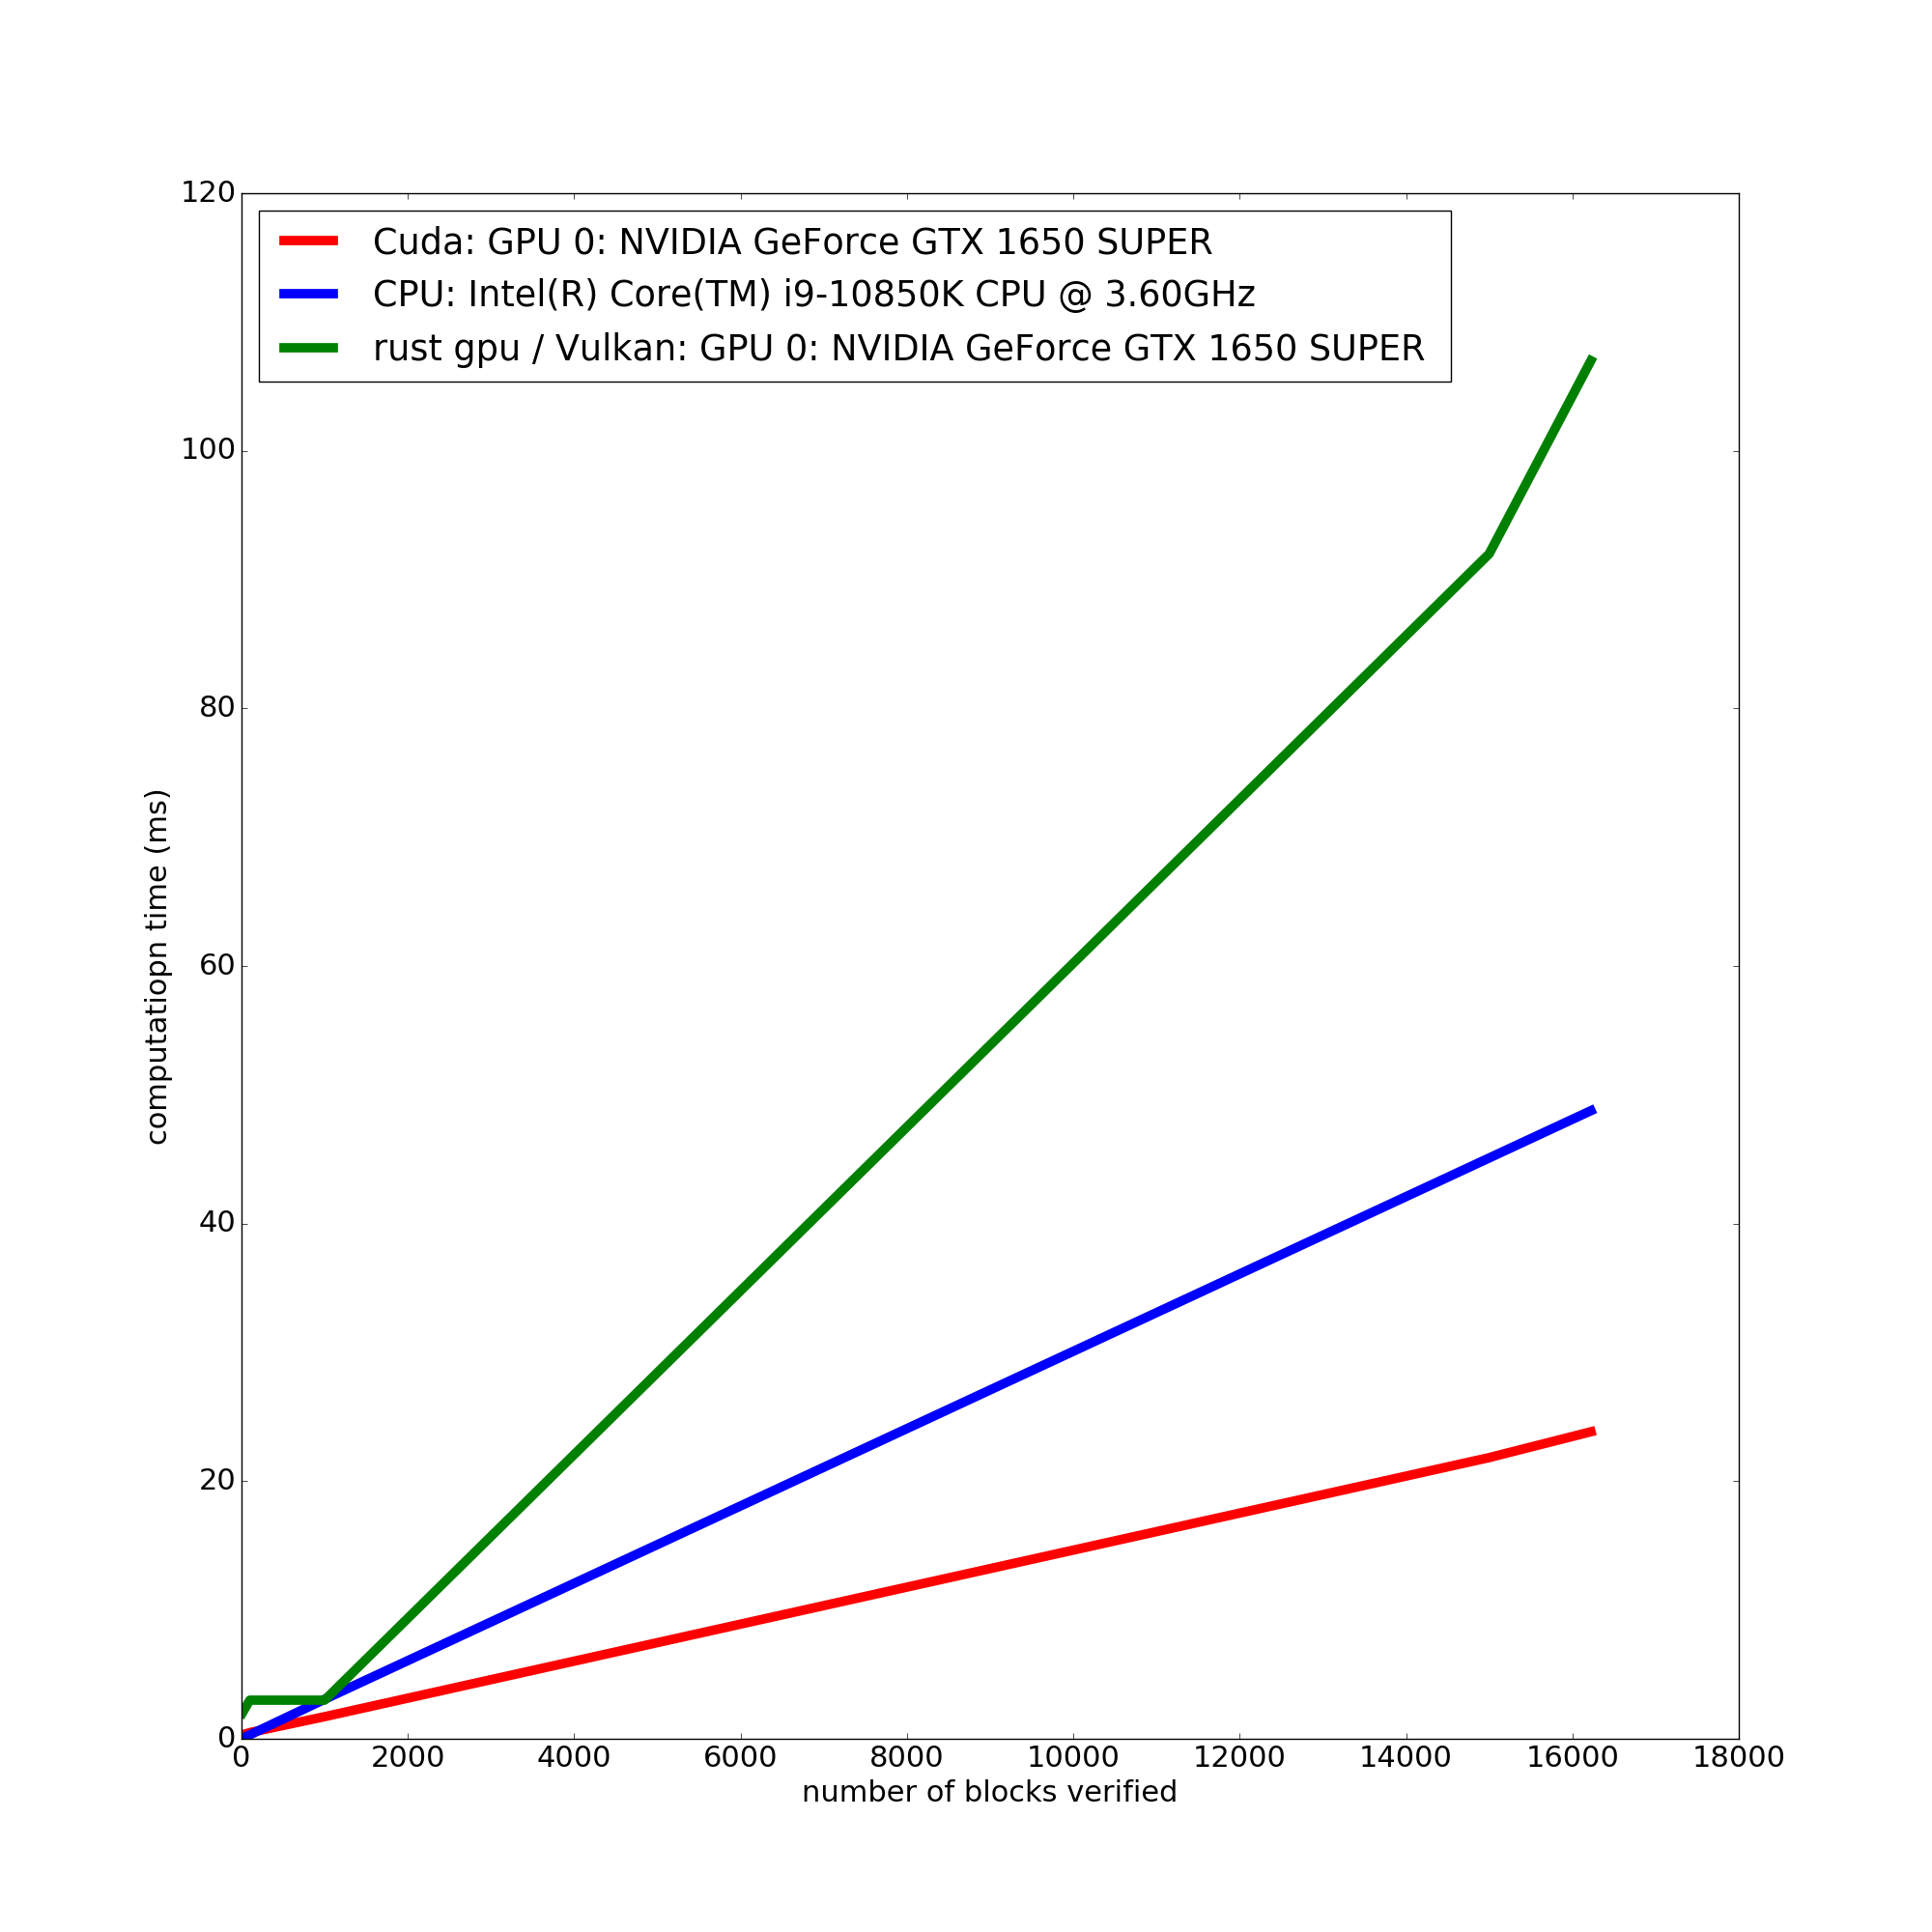
\includegraphics[width=1\linewidth]{performance_plot_mapped_buffer.png}
    \caption{Time taken to validate blocks.}
    \label{fig:my_label}
\end{figure}
\begin{figure}[H]
    \centering
    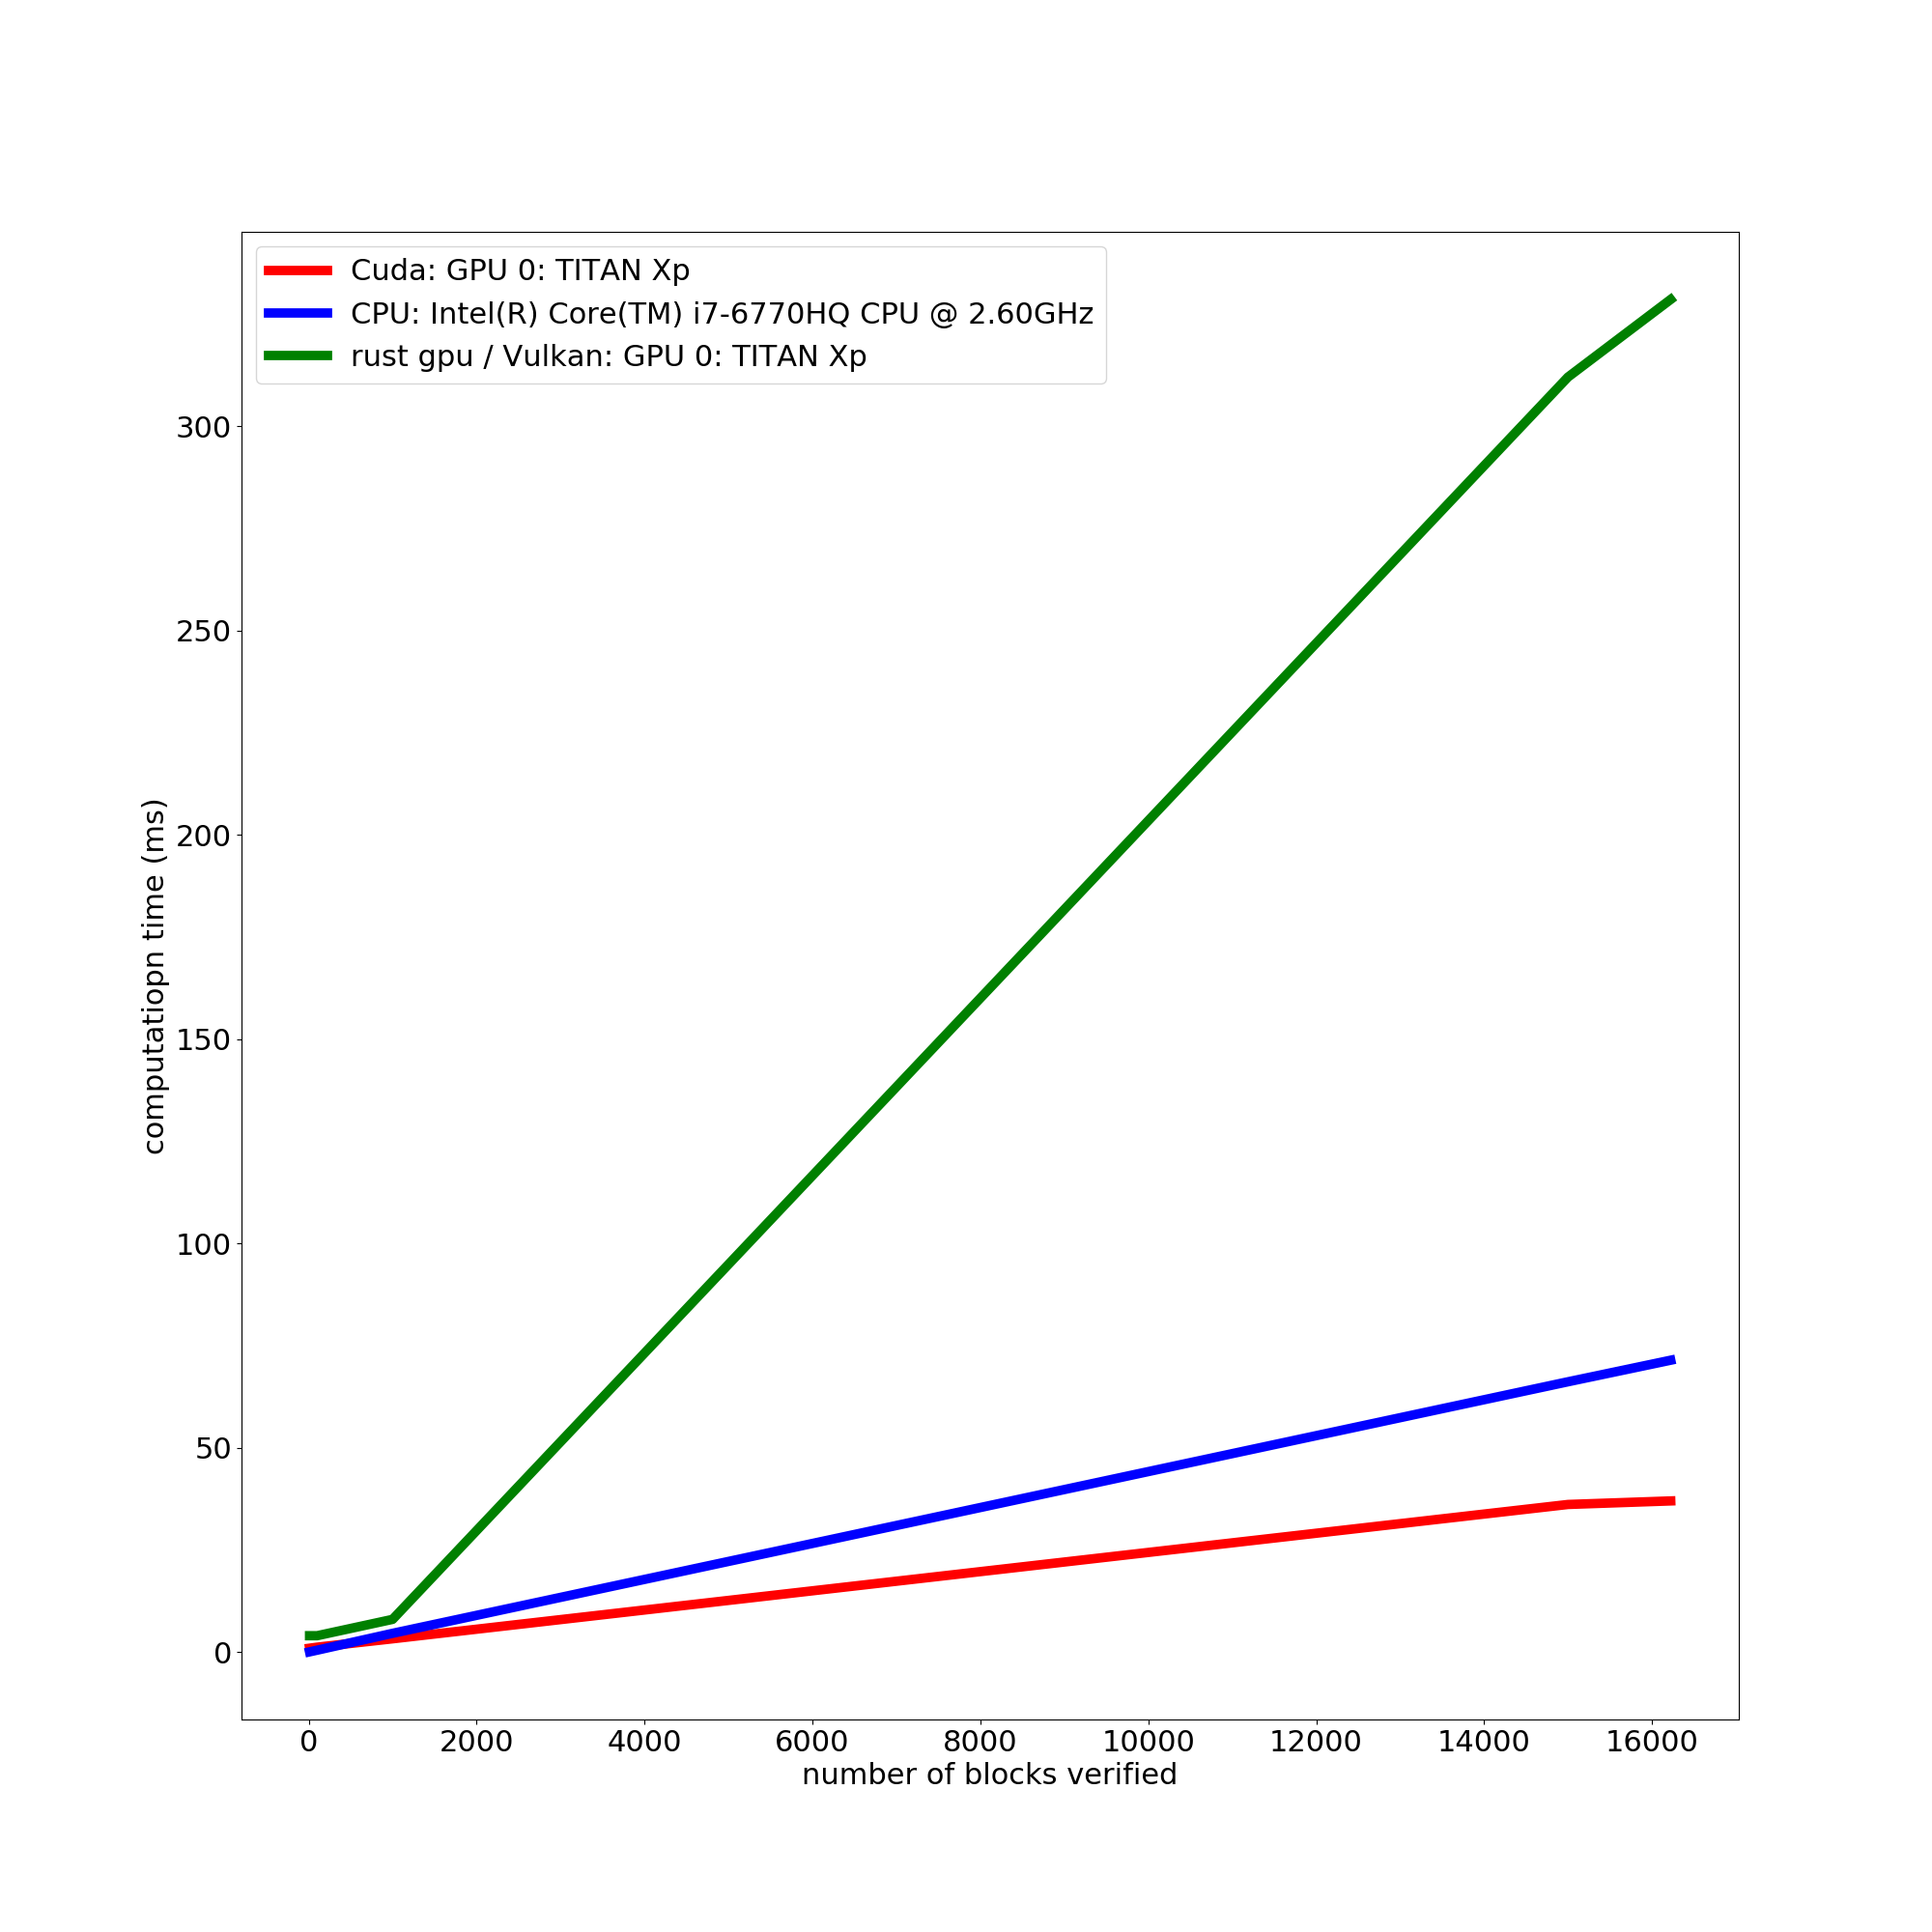
\includegraphics[width=1\linewidth]{performance_plot_titan.png}
    \caption{Time taken to validate blocks.}
    \label{fig:my_label}
\end{figure}
\begin{figure}[H]
    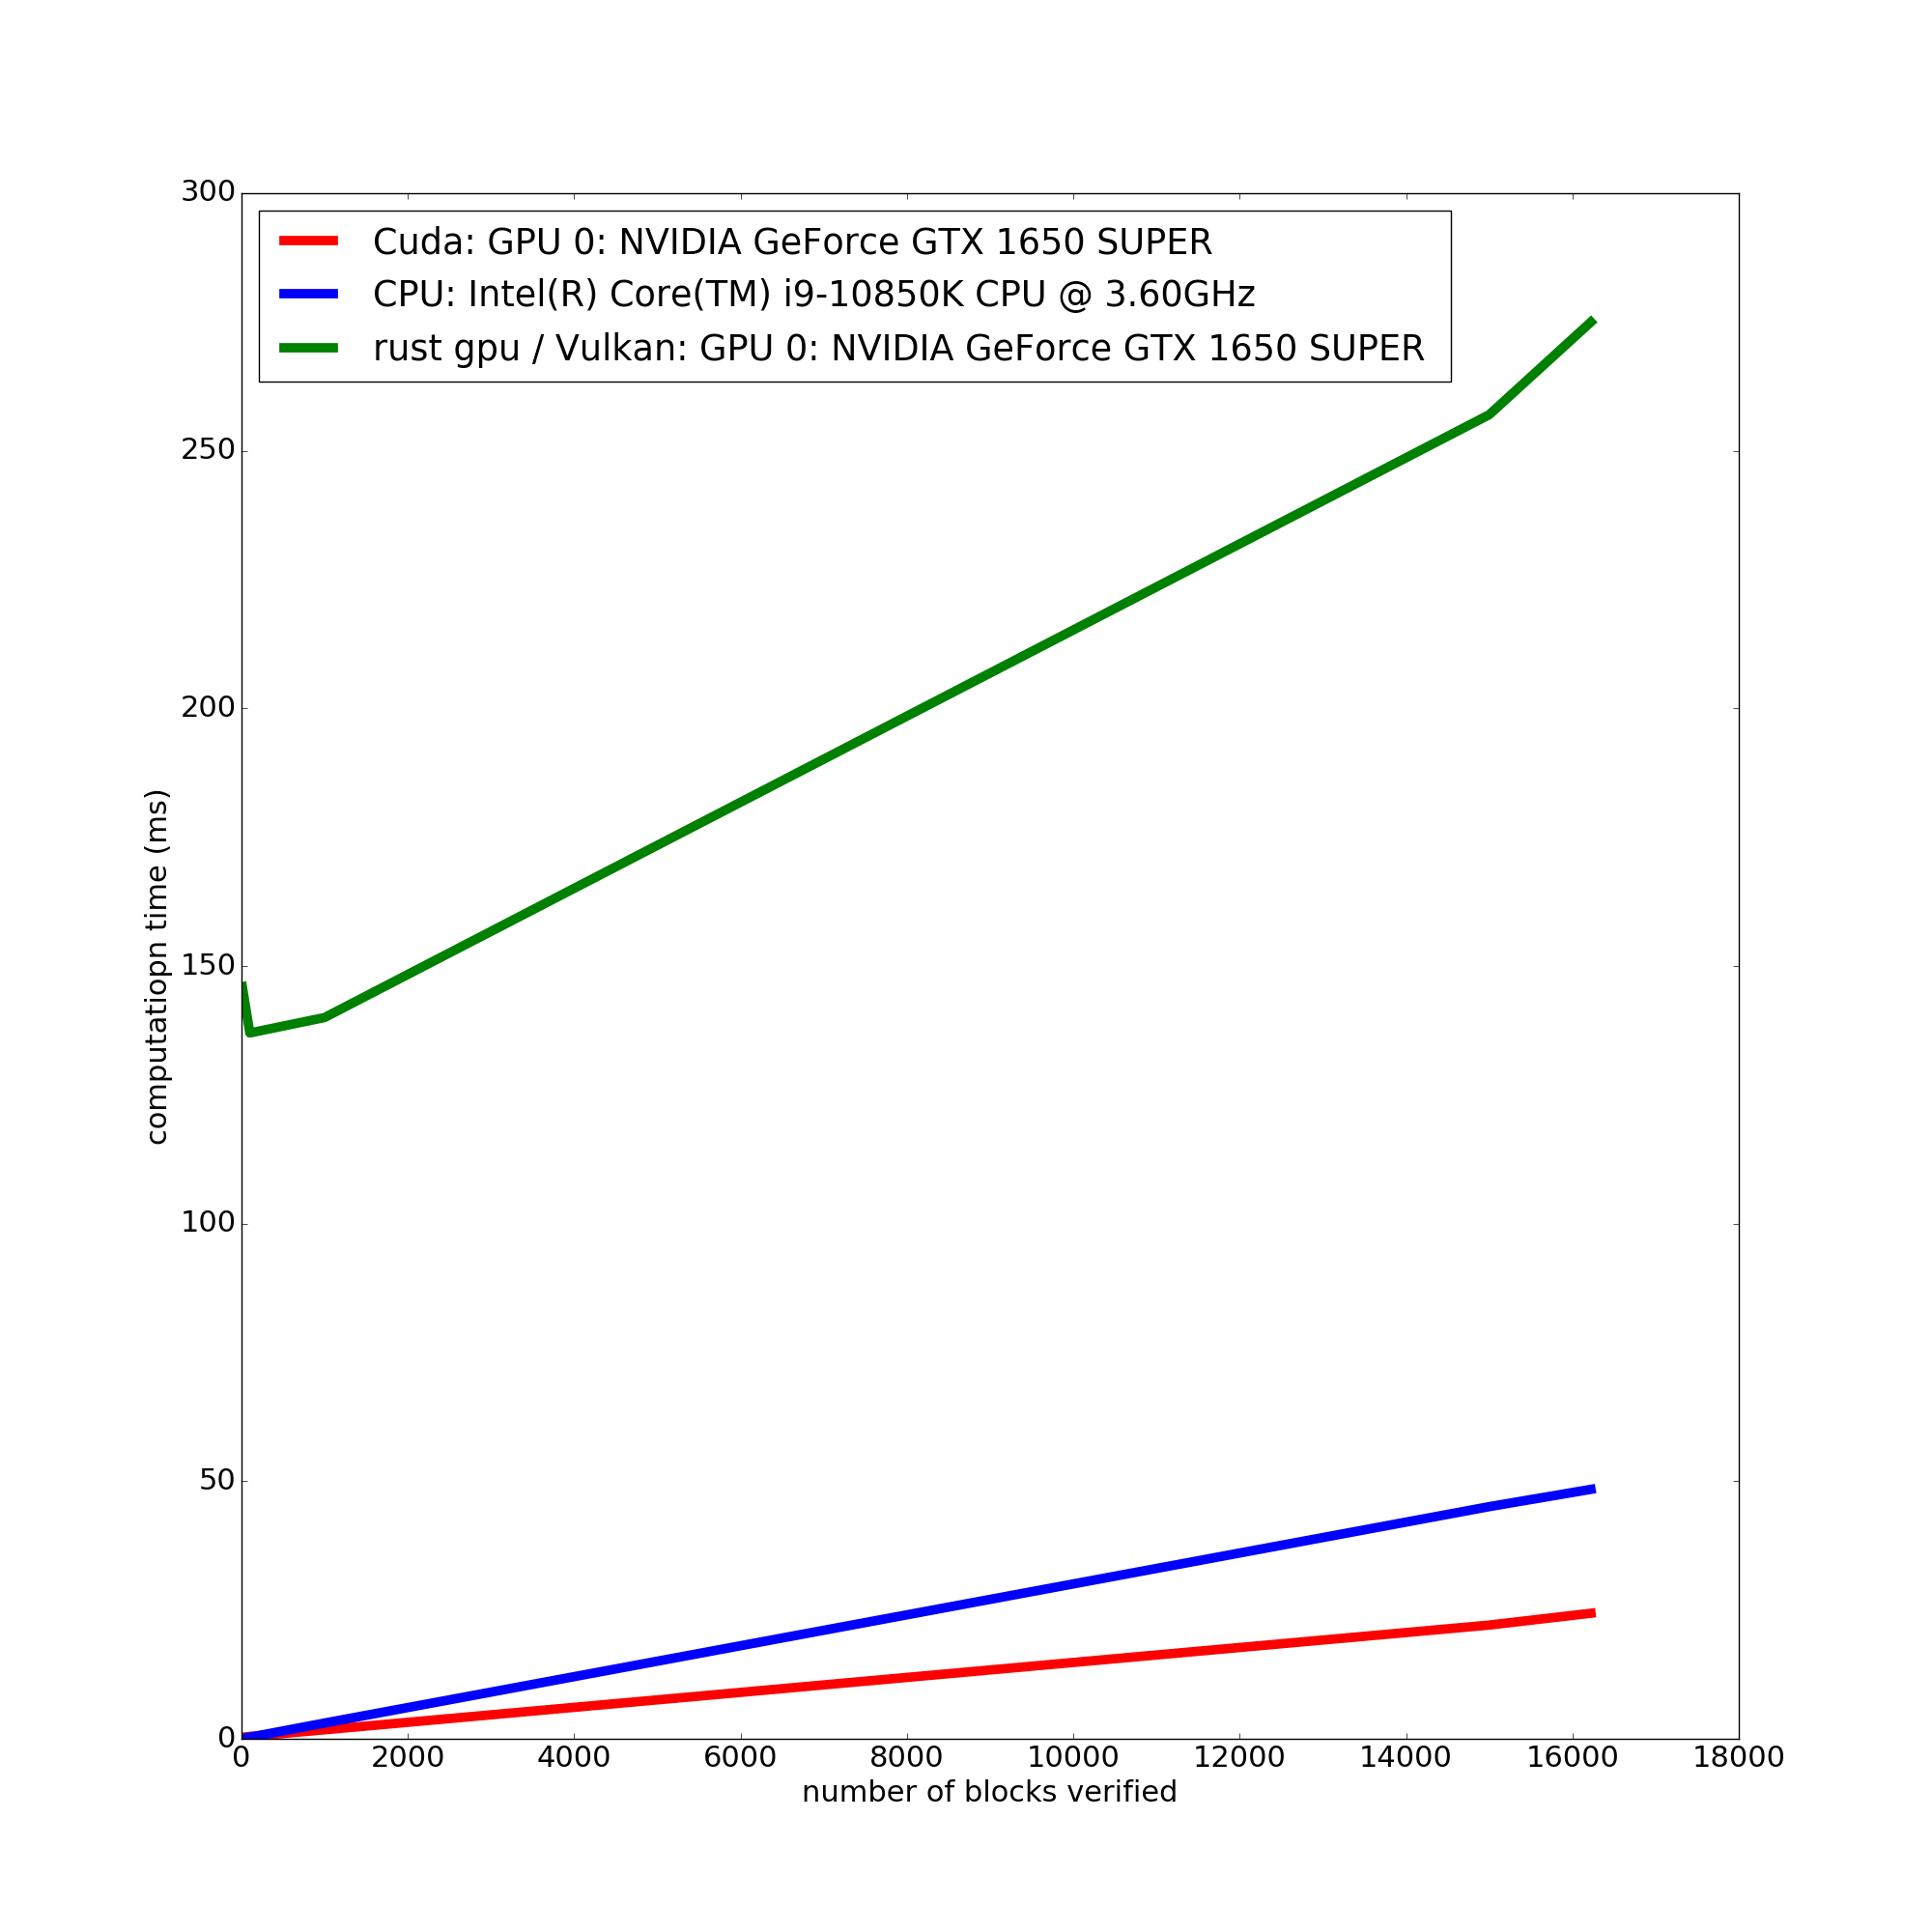
\includegraphics[width=1\linewidth]{performance_plot.png}
    \caption{Time taken to validate blocks (with Vulkan mapped memory).}
    \label{fig:my_label}
\end{figure}

\section{Code}

\subsection{CUDA/CPU}

\begin{lstlisting} [style=MyCUDAStyle]
#ifndef HASH_SHADER_SHA256_CU
#define HASH_SHADER_SHA256_CU

#include "sha256_cu.h"

__device__ int SHA256_Init(SHA256_CTX *c) {
  memset(c, 0, sizeof(*c));
  c->h[0] = 0x6a09e667UL;
  c->h[1] = 0xbb67ae85UL;
  c->h[2] = 0x3c6ef372UL;
  c->h[3] = 0xa54ff53aUL;
  c->h[4] = 0x510e527fUL;
  c->h[5] = 0x9b05688cUL;
  c->h[6] = 0x1f83d9abUL;
  c->h[7] = 0x5be0cd19UL;
  c->md_len = SHA256_DIGEST_LENGTH;
  return 1;
}

__device__ void SHA256(const unsigned char *d, size_t n, unsigned char *md) {
  SHA256_CTX c;
  SHA256_Init(&c);
  SHA256_Update(&c, d, n);
  SHA256_Final(md, &c);
  memset(&c, 0, sizeof(c));
}

#define DATA_ORDER_IS_BIG_ENDIAN

#define HASH_LONG SHA_LONG
#define HASH_CTX SHA256_CTX
#define HASH_CBLOCK SHA_CBLOCK

/*
 *  * Note that FIPS180-2 discusses "Truncation of the Hash Function Output."
 *   * default: case below covers for it. It's not clear however if it's
 *    * permitted to truncate to amount of bytes not divisible by 4. I bet not,
 *     * but if it is, then default: case shall be extended. For reference.
 *      * Idea behind separate cases for pre-defined lengths is to let the
 *       * compiler decide if it's appropriate to unroll small loops.
 *        */
#define HASH_MAKE_STRING(c, s)                                                 \
  do {                                                                         \
    unsigned long ll;                                                          \
    unsigned int nn;                                                           \
    switch ((c)->md_len) {                                                     \
    case SHA256_DIGEST_LENGTH:                                                 \
      for (nn = 0; nn < SHA256_DIGEST_LENGTH / 4; nn++) {                      \
        ll = (c)->h[nn];                                                       \
        (void)HOST_l2c(ll, (s));                                               \
      }                                                                        \
      break;                                                                   \
    default:                                                                   \
      if ((c)->md_len > SHA256_DIGEST_LENGTH)                                  \
        return 0;                                                              \
      for (nn = 0; nn < (c)->md_len / 4; nn++) {                               \
        ll = (c)->h[nn];                                                       \
        (void)HOST_l2c(ll, (s));                                               \
      }                                                                        \
      break;                                                                   \
    }                                                                          \
  } while (0)

#define HASH_UPDATE SHA256_Update
#define HASH_TRANSFORM SHA256_Transform
#define HASH_FINAL SHA256_Final
#define HASH_BLOCK_DATA_ORDER sha256_block_data_order
__device__ void sha256_block_data_order(SHA256_CTX *ctx, const void *in,
                                        size_t num);

#include "md32_common_cu.h"

#ifndef SHA256_ASM
__constant__ SHA_LONG K256[64] = {
    0x428a2f98UL, 0x71374491UL, 0xb5c0fbcfUL, 0xe9b5dba5UL, 0x3956c25bUL,
    0x59f111f1UL, 0x923f82a4UL, 0xab1c5ed5UL, 0xd807aa98UL, 0x12835b01UL,
    0x243185beUL, 0x550c7dc3UL, 0x72be5d74UL, 0x80deb1feUL, 0x9bdc06a7UL,
    0xc19bf174UL, 0xe49b69c1UL, 0xefbe4786UL, 0x0fc19dc6UL, 0x240ca1ccUL,
    0x2de92c6fUL, 0x4a7484aaUL, 0x5cb0a9dcUL, 0x76f988daUL, 0x983e5152UL,
    0xa831c66dUL, 0xb00327c8UL, 0xbf597fc7UL, 0xc6e00bf3UL, 0xd5a79147UL,
    0x06ca6351UL, 0x14292967UL, 0x27b70a85UL, 0x2e1b2138UL, 0x4d2c6dfcUL,
    0x53380d13UL, 0x650a7354UL, 0x766a0abbUL, 0x81c2c92eUL, 0x92722c85UL,
    0xa2bfe8a1UL, 0xa81a664bUL, 0xc24b8b70UL, 0xc76c51a3UL, 0xd192e819UL,
    0xd6990624UL, 0xf40e3585UL, 0x106aa070UL, 0x19a4c116UL, 0x1e376c08UL,
    0x2748774cUL, 0x34b0bcb5UL, 0x391c0cb3UL, 0x4ed8aa4aUL, 0x5b9cca4fUL,
    0x682e6ff3UL, 0x748f82eeUL, 0x78a5636fUL, 0x84c87814UL, 0x8cc70208UL,
    0x90befffaUL, 0xa4506cebUL, 0xbef9a3f7UL, 0xc67178f2UL};

/*
 *  * FIPS specification refers to right rotations, while our ROTATE macro
 *   * is left one. This is why you might notice that rotation coefficients
 *    * differ from those observed in FIPS document by 32-N...
 *     */
#define Sigma0(x) (ROTATE((x), 30) ^ ROTATE((x), 19) ^ ROTATE((x), 10))
#define Sigma1(x) (ROTATE((x), 26) ^ ROTATE((x), 21) ^ ROTATE((x), 7))
#define sigma0(x) (ROTATE((x), 25) ^ ROTATE((x), 14) ^ ((x) >> 3))
#define sigma1(x) (ROTATE((x), 15) ^ ROTATE((x), 13) ^ ((x) >> 10))

#define Ch(x, y, z) (((x) & (y)) ^ ((~(x)) & (z)))
#define Maj(x, y, z) (((x) & (y)) ^ ((x) & (z)) ^ ((y) & (z)))

__device__ inline void sha256_block_data_order(SHA256_CTX *ctx, const void *in,
                                               size_t num) {
  unsigned MD32_REG_T a, b, c, d, e, f, g, h, s0, s1, T1, T2;
  SHA_LONG X[16], l;
  int i;
  const unsigned char *data = (unsigned char *)in;

  while (num--) {
    a = ctx->h[0];
    b = ctx->h[1];
    c = ctx->h[2];
    d = ctx->h[3];
    e = ctx->h[4];
    f = ctx->h[5];
    g = ctx->h[6];
    h = ctx->h[7];

    for (i = 0; i < 16; i++) {
      (void)HOST_c2l(data, l);
      T1 = X[i] = l;
      T1 += h + Sigma1(e) + Ch(e, f, g) + K256[i];
      T2 = Sigma0(a) + Maj(a, b, c);
      h = g;
      g = f;
      f = e;
      e = d + T1;
      d = c;
      c = b;
      b = a;
      a = T1 + T2;
    }

    for (; i < 64; i++) {
      s0 = X[(i + 1) & 0x0f];
      s0 = sigma0(s0);
      s1 = X[(i + 14) & 0x0f];
      s1 = sigma1(s1);

      T1 = X[i & 0xf] += s0 + s1 + X[(i + 9) & 0xf];
      T1 += h + Sigma1(e) + Ch(e, f, g) + K256[i];
      T2 = Sigma0(a) + Maj(a, b, c);
      h = g;
      g = f;
      f = e;
      e = d + T1;
      d = c;
      c = b;
      b = a;
      a = T1 + T2;
    }

    ctx->h[0] += a;
    ctx->h[1] += b;
    ctx->h[2] += c;
    ctx->h[3] += d;
    ctx->h[4] += e;
    ctx->h[5] += f;
    ctx->h[6] += g;
    ctx->h[7] += h;
  }
}

#else

#define ROUND_00_15(i, a, b, c, d, e, f, g, h)                                 \
  do {                                                                         \
    T1 += h + Sigma1(e) + Ch(e, f, g) + K256[i];                               \
    h = Sigma0(a) + Maj(a, b, c);                                              \
    d += T1;                                                                   \
    h += T1;                                                                   \
  } while (0)

#define ROUND_16_63(i, a, b, c, d, e, f, g, h, X)                              \
  do {                                                                         \
    s0 = X[(i + 1) & 0x0f];                                                    \
    s0 = sigma0(s0);                                                           \
    s1 = X[(i + 14) & 0x0f];                                                   \
    s1 = sigma1(s1);                                                           \
    T1 = X[(i)&0x0f] += s0 + s1 + X[(i + 9) & 0x0f];                           \
    ROUND_00_15(i, a, b, c, d, e, f, g, h);                                    \
  } while (0)

__device__ inline void sha256_block_data_order(SHA256_CTX *ctx, const void *in,
                                               size_t num) {
  unsigned MD32_REG_T a, b, c, d, e, f, g, h, s0, s1, T1;
  SHA_LONG X[16];
  int i;
  const unsigned char *data = in;
  DECLARE_IS_ENDIAN;

  while (num--) {
    a = ctx->h[0];
    b = ctx->h[1];
    c = ctx->h[2];
    d = ctx->h[3];
    e = ctx->h[4];
    f = ctx->h[5];
    g = ctx->h[6];
    h = ctx->h[7];

    if (!IS_LITTLE_ENDIAN && sizeof(SHA_LONG) == 4 && ((size_t)in % 4) == 0) {
      const SHA_LONG *W = (const SHA_LONG *)data;

      T1 = X[0] = W[0];
      ROUND_00_15(0, a, b, c, d, e, f, g, h);
      T1 = X[1] = W[1];
      ROUND_00_15(1, h, a, b, c, d, e, f, g);
      T1 = X[2] = W[2];
      ROUND_00_15(2, g, h, a, b, c, d, e, f);
      T1 = X[3] = W[3];
      ROUND_00_15(3, f, g, h, a, b, c, d, e);
      T1 = X[4] = W[4];
      ROUND_00_15(4, e, f, g, h, a, b, c, d);
      T1 = X[5] = W[5];
      ROUND_00_15(5, d, e, f, g, h, a, b, c);
      T1 = X[6] = W[6];
      ROUND_00_15(6, c, d, e, f, g, h, a, b);
      T1 = X[7] = W[7];
      ROUND_00_15(7, b, c, d, e, f, g, h, a);
      T1 = X[8] = W[8];
      ROUND_00_15(8, a, b, c, d, e, f, g, h);
      T1 = X[9] = W[9];
      ROUND_00_15(9, h, a, b, c, d, e, f, g);
      T1 = X[10] = W[10];
      ROUND_00_15(10, g, h, a, b, c, d, e, f);
      T1 = X[11] = W[11];
      ROUND_00_15(11, f, g, h, a, b, c, d, e);
      T1 = X[12] = W[12];
      ROUND_00_15(12, e, f, g, h, a, b, c, d);
      T1 = X[13] = W[13];
      ROUND_00_15(13, d, e, f, g, h, a, b, c);
      T1 = X[14] = W[14];
      ROUND_00_15(14, c, d, e, f, g, h, a, b);
      T1 = X[15] = W[15];
      ROUND_00_15(15, b, c, d, e, f, g, h, a);

      data += SHA256_CBLOCK;
    } else {
      SHA_LONG l;

      (void)HOST_c2l(data, l);
      T1 = X[0] = l;
      ROUND_00_15(0, a, b, c, d, e, f, g, h);
      (void)HOST_c2l(data, l);
      T1 = X[1] = l;
      ROUND_00_15(1, h, a, b, c, d, e, f, g);
      (void)HOST_c2l(data, l);
      T1 = X[2] = l;
      ROUND_00_15(2, g, h, a, b, c, d, e, f);
      (void)HOST_c2l(data, l);
      T1 = X[3] = l;
      ROUND_00_15(3, f, g, h, a, b, c, d, e);
      (void)HOST_c2l(data, l);
      T1 = X[4] = l;
      ROUND_00_15(4, e, f, g, h, a, b, c, d);
      (void)HOST_c2l(data, l);
      T1 = X[5] = l;
      ROUND_00_15(5, d, e, f, g, h, a, b, c);
      (void)HOST_c2l(data, l);
      T1 = X[6] = l;
      ROUND_00_15(6, c, d, e, f, g, h, a, b);
      (void)HOST_c2l(data, l);
      T1 = X[7] = l;
      ROUND_00_15(7, b, c, d, e, f, g, h, a);
      (void)HOST_c2l(data, l);
      T1 = X[8] = l;
      ROUND_00_15(8, a, b, c, d, e, f, g, h);
      (void)HOST_c2l(data, l);
      T1 = X[9] = l;
      ROUND_00_15(9, h, a, b, c, d, e, f, g);
      (void)HOST_c2l(data, l);
      T1 = X[10] = l;
      ROUND_00_15(10, g, h, a, b, c, d, e, f);
      (void)HOST_c2l(data, l);
      T1 = X[11] = l;
      ROUND_00_15(11, f, g, h, a, b, c, d, e);
      (void)HOST_c2l(data, l);
      T1 = X[12] = l;
      ROUND_00_15(12, e, f, g, h, a, b, c, d);
      (void)HOST_c2l(data, l);
      T1 = X[13] = l;
      ROUND_00_15(13, d, e, f, g, h, a, b, c);
      (void)HOST_c2l(data, l);
      T1 = X[14] = l;
      ROUND_00_15(14, c, d, e, f, g, h, a, b);
      (void)HOST_c2l(data, l);
      T1 = X[15] = l;
      ROUND_00_15(15, b, c, d, e, f, g, h, a);
    }

    for (i = 16; i < 64; i += 8) {
      ROUND_16_63(i + 0, a, b, c, d, e, f, g, h, X);
      ROUND_16_63(i + 1, h, a, b, c, d, e, f, g, X);
      ROUND_16_63(i + 2, g, h, a, b, c, d, e, f, X);
      ROUND_16_63(i + 3, f, g, h, a, b, c, d, e, X);
      ROUND_16_63(i + 4, e, f, g, h, a, b, c, d, X);
      ROUND_16_63(i + 5, d, e, f, g, h, a, b, c, X);
      ROUND_16_63(i + 6, c, d, e, f, g, h, a, b, X);
      ROUND_16_63(i + 7, b, c, d, e, f, g, h, a, X);
    }

    ctx->h[0] += a;
    ctx->h[1] += b;
    ctx->h[2] += c;
    ctx->h[3] += d;
    ctx->h[4] += e;
    ctx->h[5] += f;
    ctx->h[6] += g;
    ctx->h[7] += h;
  }
}

#endif
#endif

\end{lstlisting}

\begin{lstlisting} [style=MyCUDAStyle]
#include "test.h"
#include <stdio.h>

#include "test_block_chain.h"

// linking cuda too hard
#include "sha256.cu"

char* run_sha256(unsigned char *block_buf, int *block_starts, int num_blocks);


void* pinned_alloc(size_t n) {
  void* h_aPinned = NULL;
  cudaError_t status = cudaMallocHost((void**)&h_aPinned, n);
  if (status != cudaSuccess) {
    printf("Error allocating pinned host memory\n");
    exit(-1);
  }
  return h_aPinned;
}

void pinned_free(void* p) {
  cudaFreeHost(p);
}

int main(int argc, char *argv[]) {
  if (argc < 2) {
    printf("Must have at least one argument\n");
    return -1;
  }

  test_block_chain(argv[1], argc > 2 ? atoi(argv[2]) : -1, run_sha256, pinned_alloc, pinned_free);
  return 0;
}

__global__ void kernel(unsigned char *block_buf, int *block_starts, int num_blocks, unsigned char* digests) {
  int i = threadIdx.x + blockIdx.x * blockDim.x;
  if (i < num_blocks) {
    unsigned char intermidiate_digest[SHA256_DIGEST_LENGTH];
    int front = block_starts[i];
    int back = block_starts[i+1];
    SHA256(block_buf + front, back - front, intermidiate_digest);
    __syncthreads();
    SHA256(intermidiate_digest, SHA256_DIGEST_LENGTH, digests+(i*SHA256_DIGEST_LENGTH));
  }
}

char* run_sha256(unsigned char *block_buf, int *block_starts, int num_blocks) {

  cudaDeviceSynchronize();
  unsigned char *dev_block_buf;
  cudaMallocManaged((void **)&dev_block_buf, block_starts[num_blocks]);
  cudaMemcpy(dev_block_buf, block_buf, block_starts[num_blocks], cudaMemcpyHostToDevice);

  int *dev_block_starts;
  cudaMallocManaged((void **)&dev_block_starts, sizeof(int)*(num_blocks+1));
  cudaMemcpy(dev_block_starts, block_starts, sizeof(int)*(num_blocks+1), cudaMemcpyHostToDevice);

  unsigned char *dev_digests;
  cudaMallocManaged((void **)&dev_digests, SHA256_DIGEST_LENGTH * num_blocks);
  unsigned char digests[SHA256_DIGEST_LENGTH * num_blocks] = {};

  int num_thread_blocks = (num_blocks / 256) + 1;
  dim3 threadsPerThreadBlock(256);

  kernel<<<num_thread_blocks, threadsPerThreadBlock>>>(dev_block_buf, dev_block_starts, num_blocks, dev_digests);
  cudaDeviceSynchronize();
  cudaError_t error = cudaGetLastError();
  if (error != cudaSuccess) {
    printf("CUDA error: %s\n", cudaGetErrorString(error));
    exit(-1);
  }

  cudaMemcpy(digests, dev_digests, SHA256_DIGEST_LENGTH*num_blocks, cudaMemcpyDeviceToHost);
  int res_len = (num_blocks * SHA256_DIGEST_LENGTH * 2) + num_blocks;
  char* res = (char*)malloc(res_len);
  int j = 0;
  for (int i = 0; i < num_blocks*SHA256_DIGEST_LENGTH; ++i) {
    if (i % SHA256_DIGEST_LENGTH == 0) {
      sprintf(&res[j], " ");
      j += 1;
    }
    sprintf(&res[j], "%02x", digests[i]);
    j += 2;
  }
  cudaFree(dev_block_buf);
  cudaFree(dev_block_starts);
  cudaFree(dev_digests);
  return res;
}

\end{lstlisting}


\subsection{Vulkan}

\begin{lstlisting}[language=Rust, style=boxed]
#![allow(non_snake_case)]
#![cfg_attr(
    target_arch = "spirv",
    no_std,
    feature(register_attr),
    register_attr(spirv)
)]

#[cfg(not(target_arch = "spirv"))]
#[macro_use]
pub extern crate spirv_std_macros;

use glam::UVec3;

// Rotation right: u32.rotate_right(n: u32)
fn rot_r(x: u32, n: u32) -> u32 {
    x >> n | (x << (32 - n))
}

fn Sigma0(x: u32) -> u32 {
    rot_r(x, 2) ^ rot_r(x, 13) ^ rot_r(x, 22)
    //x.rotate_right(2) ^ x.rotate_right(13) ^ x.rotate_right(22)
}
#[test]
fn test_Sigma0() {
    let x: u32 = 0b00000000000000000011111111111111;
    let y: u32 = 0b00111111000001111111001111111110;
    let r = Sigma0(x);
    assert_eq!(
        r, y,
        "Testing choice:\n x:{:#034b}\n y:{:#034b}\n e:{:#034b}",
        x, y, r
    );
}

fn Sigma1(x: u32) -> u32 {
    rot_r(x, 6) ^ rot_r(x, 11) ^ rot_r(x, 25)
    //x.rotate_right(6) ^ x.rotate_right(11) ^ x.rotate_right(25)
}
#[test]
fn test_Sigma1() {
    let x: u32 = 0b00000000000000000011111111111111;
    let y: u32 = 0b00000011111111111111111101111000;
    let r = Sigma1(x);
    assert_eq!(
        r, y,
        "Testing choice:\n x:{:#034b}\n y:{:#034b}\n e:{:#034b}",
        x, y, r
    );
}
fn sigma0(x: u32) -> u32 {
    rot_r(x, 7) ^ rot_r(x, 18) ^ (x >> 3)
    //x.rotate_right(7) ^ x.rotate_right(18) ^ (x >> 3)
}
#[test]
fn test_sigma0() {
    let x: u32 = 0b00000000000000000011111111111111;
    let y: u32 = 0b11110001111111111100011110000000;
    let r = sigma0(x);
    assert_eq!(
        r, y,
        "Testing choice:\n x:{:#034b}\n y:{:#034b}\n e:{:#034b}",
        x, y, r
    );
}

fn sigma1(x: u32) -> u32 {
    rot_r(x, 17) ^ rot_r(x, 19) ^ (x >> 10)
    //x.rotate_right(17) ^ x.rotate_right(19) ^ (x >> 10)
}
#[test]
fn test_sigma1() {
    let x: u32 = 0b00000000000000000011111111111111;
    let y: u32 = 0b00011000000000000110000000001111;
    let r = sigma1(x);
    assert_eq!(
        r, y,
        "Testing choice:\n x:{:#034b}\n y:{:#034b}\n e:{:#034b}",
        x, y, r
    );

    let x: u32 = 0b00000000000000000000000000011000;
    let y: u32 = 0b00000000000011110000000000000000;
    let r = sigma1(x);
    assert_eq!(
        r, y,
        "Testing choice:\n x:{:#034b}\n y:{:#034b}\n e:{:#034b}",
        x, y, r
    );
}

// Choice operation
fn ch(x: u32, y: u32, z: u32) -> u32 {
    (x & y) ^ (!x & z)
}

#[test]
fn test_ch() {
    let x: u32 = 0b0000000111111110000000011111111;
    let y: u32 = 0b0000000000000001111111111111111;
    let z: u32 = 0b1111111111111110000000000000000;
    let w: u32 = 0b1111111000000000000000011111111;
    assert_eq!(
        ch(x, y, z),
        w,
        "Testing choice:\n x:{:#034b}\n y:{:#034b}\n z:{:#034b}\n w:{:#034b}",
        x,
        y,
        z,
        w
    );
}

// Majority operation
fn maj(x: u32, y: u32, z: u32) -> u32 {
    (x & y) ^ (x & z) ^ (y & z)
}

#[test]
fn test_maj() {
    let x: u32 = 0b0000000111111110000000011111111;
    let y: u32 = 0b0000000000000001111111111111111;
    let z: u32 = 0b1111111111111110000000000000000;
    let w: u32 = 0b0000000111111110000000011111111;
    assert_eq!(
        maj(x, y, z),
        w,
        "Testing choice:\n x:{:#034b}\n y:{:#034b}\n z:{:#034b}\n w:{:#034b}",
        x,
        y,
        z,
        w
    );
}

const K: [u32; 64] = [
    0x428a2f98, 0x71374491, 0xb5c0fbcf, 0xe9b5dba5, 0x3956c25b, 0x59f111f1, 0x923f82a4, 0xab1c5ed5,
    0xd807aa98, 0x12835b01, 0x243185be, 0x550c7dc3, 0x72be5d74, 0x80deb1fe, 0x9bdc06a7, 0xc19bf174,
    0xe49b69c1, 0xefbe4786, 0x0fc19dc6, 0x240ca1cc, 0x2de92c6f, 0x4a7484aa, 0x5cb0a9dc, 0x76f988da,
    0x983e5152, 0xa831c66d, 0xb00327c8, 0xbf597fc7, 0xc6e00bf3, 0xd5a79147, 0x06ca6351, 0x14292967,
    0x27b70a85, 0x2e1b2138, 0x4d2c6dfc, 0x53380d13, 0x650a7354, 0x766a0abb, 0x81c2c92e, 0x92722c85,
    0xa2bfe8a1, 0xa81a664b, 0xc24b8b70, 0xc76c51a3, 0xd192e819, 0xd6990624, 0xf40e3585, 0x106aa070,
    0x19a4c116, 0x1e376c08, 0x2748774c, 0x34b0bcb5, 0x391c0cb3, 0x4ed8aa4a, 0x5b9cca4f, 0x682e6ff3,
    0x748f82ee, 0x78a5636f, 0x84c87814, 0x8cc70208, 0x90befffa, 0xa4506ceb, 0xbef9a3f7, 0xc67178f2,
];

#[test]
fn test_K() {
    let primes = vec![
        2, 3, 5, 7, 11, 13, 17, 19, 23, 29, 31, 37, 41, 43, 47, 53, 59, 61, 67, 71, 73, 79, 83, 89,
        97, 101, 103, 107, 109, 113, 127, 131, 137, 139, 149, 151, 157, 163, 167, 173, 179, 181,
        191, 193, 197, 199, 211, 223, 227, 229, 233, 239, 241, 251, 257, 263, 269, 271, 277, 281,
        283, 293, 307, 311,
    ];
    for (ix, n) in primes.into_iter().enumerate() {
        // Get the fractional part as hex
        let mut fractional = (n as f64).cbrt().fract();
        let mut hex = [0u8; 8];
        for h in 0..hex.len() {
            let product = fractional * 16.;
            let carry = product.floor() as u8;
            fractional = product - product.floor();
            hex[h] = carry;
        }
        // Convert the hex array (4 bits but represented as u8) to a u32
        let mut value: u32 = hex[7] as u32;
        for (i, h) in (0..hex.len() - 1).rev().enumerate() {
            value += hex[h] as u32 * 16_u32.pow(i as u32 + 1);
        }
        assert_eq!(K[ix], value);
    }
}

const INIT_HASH: [u32; 8] = [
    0x6a09e667, 0xbb67ae85, 0x3c6ef372, 0xa54ff53a, 0x510e527f, 0x9b05688c, 0x1f83d9ab, 0x5be0cd19,
];

fn hash_fn(text: &[u32], hash: &mut [u32], x: usize, offset: usize, iter: usize) {
    // Offsets for loading and storing in data buffers
    let load_offset = (iter + x + offset) * 16;
    let store_offset = x * 8;

    let (mut a, mut b, mut c, mut d, mut e, mut f, mut g, mut h, mut t1, mut t2): (
        u32,
        u32,
        u32,
        u32,
        u32,
        u32,
        u32,
        u32,
        u32,
        u32,
    );

    // Need to manually unroll declaration
    let mut m: [u32; 64] = [
        0, 0, 0, 0, 0, 0, 0, 0, 0, 0, 0, 0, 0, 0, 0, 0, 0, 0, 0, 0, 0, 0, 0, 0, 0, 0, 0, 0, 0, 0,
        0, 0, 0, 0, 0, 0, 0, 0, 0, 0, 0, 0, 0, 0, 0, 0, 0, 0, 0, 0, 0, 0, 0, 0, 0, 0, 0, 0, 0, 0,
        0, 0, 0, 0,
    ];

    // Create the message schedule
    // The first 16 are assumed to be given
    for i in 0..16 {
        m[i] = text[load_offset + i];
    }

    // Compute the remaining message schedule
    for i in 16..64 {
        m[i] = sigma1(m[i - 2]) + m[i - 7] + sigma0(m[i - 15]) + m[i - 16];
        //println!("{} {:#034b}", i, m[i]);
    }

    // Do compression
    // The initial hash value as sqrt of primes
    if iter == 0 {
        a = INIT_HASH[0];
        b = INIT_HASH[1];
        c = INIT_HASH[2];
        d = INIT_HASH[3];
        e = INIT_HASH[4];
        f = INIT_HASH[5];
        g = INIT_HASH[6];
        h = INIT_HASH[7];
    } else {
        a = hash[store_offset + 0];
        b = hash[store_offset + 1];
        c = hash[store_offset + 2];
        d = hash[store_offset + 3];
        e = hash[store_offset + 4];
        f = hash[store_offset + 5];
        g = hash[store_offset + 6];
        h = hash[store_offset + 7];
    }

    for i in 0..64 {
        t1 = Sigma1(e) + ch(e, f, g) + h + K[i] + m[i];
        t2 = Sigma0(a) + maj(a, b, c);
        h = g;
        g = f;
        f = e;
        e = d + t1;
        d = c;
        c = b;
        b = a;
        a = t1 + t2;
    }

    // Add the original hashed message with initial hash
    if iter == 0 {
        a += INIT_HASH[0];
        b += INIT_HASH[1];
        c += INIT_HASH[2];
        d += INIT_HASH[3];
        e += INIT_HASH[4];
        f += INIT_HASH[5];
        g += INIT_HASH[6];
        h += INIT_HASH[7];
    } else {
        a += hash[store_offset + 0];
        b += hash[store_offset + 1];
        c += hash[store_offset + 2];
        d += hash[store_offset + 3];
        e += hash[store_offset + 4];
        f += hash[store_offset + 5];
        g += hash[store_offset + 6];
        h += hash[store_offset + 7];
    }

    // Store result
    hash[store_offset + 0] = a;
    hash[store_offset + 1] = b;
    hash[store_offset + 2] = c;
    hash[store_offset + 3] = d;
    hash[store_offset + 4] = e;
    hash[store_offset + 5] = f;
    hash[store_offset + 6] = g;
    hash[store_offset + 7] = h;
}

#[test]
fn test_hash_fn() {
    let word: String = String::from("abc");
    let mut init: Vec<u8> = word.into_bytes();

    let msg_size = (init.len() * 8) as u64; // in bits

    // Add a 1 as a delimiter
    init.push(0x80 as u8);
    let size: usize = (448u32 / 8u32 - init.len() as u32) as usize;

    // Pad with zeros
    let remaining = vec![0u8; size];
    init.extend(&remaining);

    // Make the last 64 bits be the size
    let size = (msg_size).to_be_bytes();
    init.extend(&size);

    let mut text = Vec::new();

    use std::convert::TryInto;
    for i in 0..16 {
        let val = u32::from_be_bytes(init[i * 4..(i + 1) * 4].try_into().unwrap());
        text.push(val);
    }

    let mut hash = vec![0u32; 8];

    hash_fn(text.as_slice(), hash.as_mut_slice(), 0, 0, 0);

    let result: String = hash.into_iter().map(|x| format!("{:x}", x)).collect();
    assert_eq!(
        result,
        "ba7816bf8f01cfea414140de5dae2223b00361a396177a9cb410ff61f20015ad"
    );
}

#[allow(unused_attributes)]
#[spirv(compute(threads(1)))]
pub fn main_cs(
    #[spirv(global_invocation_id)] gid: UVec3,
    #[spirv(storage_buffer, descriptor_set = 0, binding = 0)] text: &[u32],
    #[spirv(storage_buffer, descriptor_set = 0, binding = 1)] hash: &mut [u32],
    #[spirv(storage_buffer, descriptor_set = 0, binding = 2)] iter: &[u32],
) {
    // The sha specification loops in blocks of 512
    let num_loops: usize = iter[gid.x as usize] as usize;

    // Calculate where the memory offset for each kernel instance
    // which depends upon the number of iterations required by all previous
    // kernel invocations
    let mut offset = 0;
    for i in 0..gid.x as usize {
        offset += iter[i] as usize - 1;
    }

    for i in 0..num_loops {
        hash_fn(text, hash, gid.x as usize, offset, i);
    }
}

\end{lstlisting}

\begin{lstlisting}[language=Rust, style=boxed]
use alkomp;

use std::env;
use std::time::{Duration, Instant};

/// Prepare the text data for GPU by padding the bits to multiples of 512
/// - Append 1 as a delimiter
/// - Append 0s
/// - The last 64 bits denote the size of original message
fn prepare_for_gpu(word: String) -> (Vec<u32>, u32) {
    let mut init: Vec<u8> = hex::decode(word).expect("Input was not hex");

    let msg_size = (init.len() * 8) as u64; // in bits

    let desired_size = (msg_size / 512 + 1) * 512;

    // Add a 1 as a delimiter
    init.push(0x80 as u8);
    let size: usize = ((desired_size - 64) as u32 / 8u32 - init.len() as u32) as usize;

    // Pad with zeros
    let remaining = vec![0u8; size];
    init.extend(&remaining);

    // Make the last 64 bits be the size
    let size = (msg_size).to_be_bytes();
    init.extend(&size);

    let mut text = Vec::new();

    use std::convert::TryInto;
    for i in 0..(desired_size / 32) as usize {
        let val = u32::from_be_bytes(init[i * 4..(i + 1) * 4].try_into().unwrap());
        text.push(val);
    }

    (text, (desired_size / 512) as u32)
}

fn sha<'a>(words: Vec<String>) -> (Box<[u32]>, Duration) {
    let count = words.len();

    // A Vec of bit strings, and a vec of "number of iterations"
    let (texts, sizes): (Vec<Vec<u32>>, Vec<u32>) =
        words.into_iter().map(|x| prepare_for_gpu(x)).unzip();

    let texts: Vec<u32> = texts.into_iter().flatten().collect();

    let hash = vec![0u32; count * 8];

    // Check number of bits
    assert_eq!(hash.len() * core::mem::size_of::<u32>() * 8, 8 * 32 * count);

    let mut device = alkomp::Device::new(0);

    let text_gpu = device.to_device(texts.as_slice());
    let hash_gpu = device.to_device(hash.as_slice());
    let size_gpu = device.to_device(sizes.as_slice());

    let shader = wgpu::include_spirv!(env!("kernel.spv"));

    let args = alkomp::ParamsBuilder::new()
        .param(Some(&text_gpu))
        .param(Some(&hash_gpu))
        .param(Some(&size_gpu))
        .build(Some(0));

    let start_1 = Instant::now();
    let compute = device.compile("main_cs", &shader, &args.0).unwrap();

    device.call(compute, (count as u32, 1, 1), &args.1);

    let hash_res = futures::executor::block_on(device.get(&hash_gpu)).unwrap();
    let duration_1 = start_1.elapsed();
    (hash_res, duration_1)
}

fn main() {
    let paths: Vec<String> = env::args().skip(1).collect();
    if paths.len() == 0 {
        println!("Input path to CSV file containing blockchain data");
        return;
    }
    let max_blocks : i32;
    if paths.len() > 1 { max_blocks = paths[1].parse().unwrap() } else { max_blocks =  -1; }

    let mut rdr = csv::Reader::from_path(&paths[0]).expect("Failed to open file");

    let mut words = Vec::new();
    let mut expected = Vec::new();

    let mut i = 0;
    for record in rdr.records() {
        if max_blocks != -1 && i == max_blocks {
            break;
        }
        let record = record.expect("Failed");
        words.push(record[0].to_string());
        expected.push(record[1].to_string());
        i += 1;
    }

    // ROUND 1 OF SHA

    let (hash_res, duration_1) = sha(words);
    let hash_res = &hash_res;

    let result: String = hash_res.into_iter().map(|x| format!("{:08x}", x)).collect();
    let chunks = result
        .as_bytes()
        .chunks(64)
        .map(std::str::from_utf8)
        .collect::<Result<Vec<&str>, _>>()
        .unwrap();

    let words = chunks.into_iter().map(|s| s.to_string()).collect();

    // ROUND 2 OF SHA

    let (hash_res, duration_2) = sha(words);
    let hash_res = &hash_res;

    let result: String = hash_res.into_iter().map(|x| format!("{:08x}", x)).collect();
    let chunks = result
        .as_bytes()
        .chunks(64)
        .map(std::str::from_utf8)
        .collect::<Result<Vec<&str>, _>>()
        .unwrap();

    for c in 0..chunks.len() {
        assert_eq!(expected[c], chunks[c]);
    }
    print!("{} {}", chunks.len(), (duration_1 + duration_2).as_millis());
}
\end{lstlisting}



\end{document}
